\documentclass[11pt]{article}

% ====================================================
% ====================================================
% USEPACKAGES AND IMPORTS
% ====================================================
% ====================================================

\usepackage[T1]{fontenc}
\usepackage[utf8]{inputenc}
\usepackage[english]{babel}

\usepackage{fancyhdr}

% definitions
% ====================================================
\let\titleoriginal\title
\renewcommand{\title}[1]{
	\titleoriginal{#1}
	\newcommand{\thetitle}{#1}
}

\setlength{\parskip}{\baselineskip}%
\setlength{\parindent}{0pt}%

% header and footer
\pagestyle{fancy}
\fancyhf{}
\lhead{Applied Machine Learning Fundamentals}
\rhead{\thetitle}
\cfoot{\thepage}

% ====================================================
% ====================================================
% PRESENTATION DATA
% ====================================================
% ====================================================

\title[Machine Learning Introduction]{*** Applied Machine Learning Fundamentals *** Machine Learning Introduction}
\institute{SAP\,SE}
\author{Daniel Wehner}
\date{\today}
\prefix{INTRO}

% ====================================================
% ====================================================
% BEGIN OF DOCUMENT
% ====================================================
% ====================================================

\begin{document}

% Title frame
%______________________________________________________________________
\maketitlepage


% Agenda
%______________________________________________________________________
\begin{frame}{Agenda \today}
	\begin{multicols}{2}
		\tableofcontents
	\end{multicols}
\end{frame}


% Section: General Overview
%______________________________________________________________________

\section{General Overview}
\makedivider{General Overview}

% Why Machine Learning?
\begin{frame}{Why Machine Learning?}{}
	\begin{itemize}
		\item \textit{`We are drowning in information and starving for knowledge.' \\
			\hfill\textbf{-- John Naisbitt}}
		\item \textbf{Era of big data:}
		\begin{itemize}
			\item In 2017 there are about \textbf{1.8 trillion} web-pages on the internet
			\item \textbf{20 hours} of video are uploaded to YouTube every minute
			\item Walmart handles more than \textbf{1 million} transactions per hour and has data bases containing more 
				than \textbf{2.5 peta-bytes} ($2.5 \times 10^15$) of information
		\end{itemize}
		\item \Highlight{No human being can deal with this data avalanche!}
	\end{itemize}
\end{frame}


% Why Machine Learning? (Ctd.)
\begin{frame}{Why Machine Learning? (Ctd.)}{}
	\textit{`I keep saying the sexy job in the next ten years will be \textbf{statisticians} and \textbf{machine learners}.
		People think I’m joking, but who would’ve guessed that computer engineers would’ve been the sexy job of the
		1990s? The ability to take data - to be able to understand it, to process it, to extract value from it, to visualize it,
		to communicate it - that’s going to be a hugely important skill in the next decades.' \\
		\hfill\textbf{-- Hal Varian}, Chief Economist at Google, 2009}
\end{frame}


% Definition of Machine Learning
\begin{frame}{Definition of Machine Learning}{}
	\begin{itemize}
		\item \textit{`[Machine Learning is the] field of study that gives computers the ability
			to learn without being explicitly programmed.' \\
			\hfill\textbf{-- Arthur Samuel}, 1959}
		\vspace*{5mm}
		\item \textit{`A computer program is said to learn from experience $E$ with respect to some class of 
			tasks $T$ and performance measure $P$, if its performance at tasks in $T$, as measured by $P$, improves with
			experience $E$.' \\
			\hfill\textbf{-- Tom Mitchell}, 1997}
	\end{itemize}
\end{frame}


% Section: Problem Types in Machine Learning
%______________________________________________________________________

\section{Problem Types in Machine Learning}
\makedivider{Problem Types in Machine Learning}

\begin{frame}{}{}

\end{frame}

\subsection{}


% Section: Key Challenges in Machine Learning
%______________________________________________________________________

\section{Key Challenges in Machine Learning}
\makedivider{Key Challenges in Machine Learning}

\begin{frame}{}{}

\end{frame}


% Section: Lecture Overview
%______________________________________________________________________

\section{Lecture Overview}
\makedivider{Lecture Overview}

\makeoverview{1}


% Section: Wrap-Up
%______________________________________________________________________

\section{Wrap-Up}
\subsection{Summary}

% Summary
\begin{frame}{Summary}{}

\end{frame}


\subsection{Recommended Literature and further Reading}

% Literature
%______________________________________________________________________
\begin{frame}{Recommended Literature and further Reading}{}
	\footnotesize
	\begin{thebibliography}{2}
		\literature{book}{Mitchell.1997}{[1] Machine Learning}
			{Tom Mitchell. McGraw-Hill Science. 1997.}{$\rightarrow$ See chapter 1 (Introduction)}
	\end{thebibliography}
\end{frame}


% Thank you
%______________________________________________________________________
\makethanks


%\section{Notation}
%
%% Notation
%\begin{frame}{Notation}
%	\begin{itemize}
%		\item Mathematical notation:
%		\begin{itemize}
%			\item Scalars: Standard letters, e.\,g. $h$, $t$, ...
%			\item Vectors: Bold-faced letters, e.\,g. $\bm{x}$, $\bm{\theta}$, ...
%			\item Matrices: Bold-faced capital letters, e.\,g. $\bm{W}$, $\bm{\Phi}$, ...
%		\end{itemize}
%		\item Symbols:
%	\end{itemize}
%
%	\begin{table}
	\scalebox{0.7}{
	\begin{tabular}{| c | l |}
		\hline
		\textbf{Symbol} 					& \textbf{Explanation} 				\\ \hline\hline
		$\alpha$ 						& Learning rate		 				\\ \hline
		$\bm{\theta}$					& Model parameters to be estimated	\\ \hline
		$\ell$							& Loss function 						\\ \hline
		$\mathcal{J}$					& Cumulated loss						\\ \hline
		$\nabla f(\bm{x})$ 				& Gradient of function $f$				\\ \hline
		$\langle \bullet, \bullet \rangle$	& Scalar product				\\ \hline
	\end{tabular}}		
\end{table}
%\end{frame}
%
%
%\section{ML Introduction}
%\makedivider{ML Introduction}
%
%\subsection{Machine Learning Terminology}
%
%% Why Machine Learning?
%\begin{frame}{Why Machine Learning?}{}
%	\begin{itemize}
%		\item Subset of artificial intelligence
%		\item The term `Machine Learning' was coined by Arthur Samuel in 1959
%		\item Machine learning explores the study and construction of algorithms that can \highlight{learn} from and
%			\highlight{make predictions on data}
%		\item Era of big data $\Rightarrow$ \textbf{no human can deal with the data avalanche}
%	\end{itemize}
%
%	\begin{boxBlue}
%		\textit{`We are drowning in information and starving for knowledge.' \\
%		\null\hfill \textbf{-- John Naisbitt}}
%	\end{boxBlue}
%\end{frame}
%
%
%\subsection{Dimension: Type of Training Information}
%
%% Type of Training Information
%\begin{frame}{Dimension: Type of Training Information}{}
%	\begin{itemize}
%		\item \highlight{Supervised Learning}
%		\begin{itemize}
%			\item A `teacher' provides values for the target function (Labeled training examples)
%			\item \textbf{E.\,g.} Neural networks, decision trees, regression, ...
%		\end{itemize}
%		\item \highlight{Unsupervised Learning}
%		\begin{itemize}
%			\item The labels are \textbf{not} known
%			\item \textbf{E.\,g.} Clustering, Apriori, ...
%		\end{itemize}
%		\item \highlight{Reinforcement Learning}
%		\begin{itemize}
%			\item A `teacher' provides rewards for actions but the correct solution is not known
%			\item \textbf{E.\,g.} Policy-Iteration, Q-Learning, SARSA
%		\end{itemize}
%		\item Semi-Supervised Learning (Examples are partly labeled, \textit{not covered})
%	\end{itemize}
%\end{frame}
%
%
%% Dimension: Type of Training Information visualized
%\begin{frame}{Dimension: Type of Training Information visualized}{}
%	\begin{figure}
	\centering
	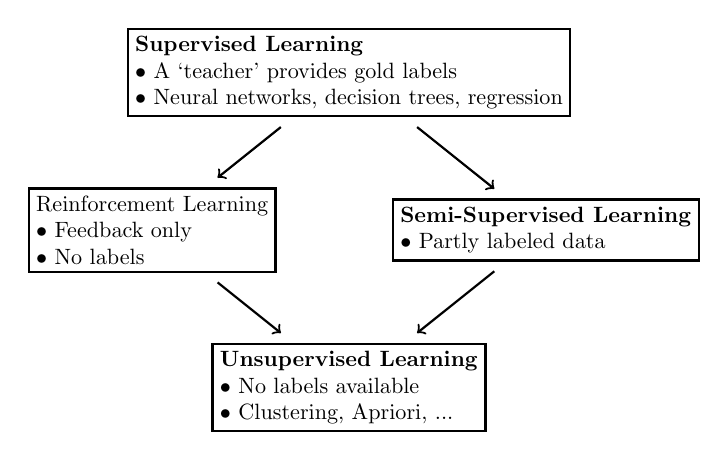
\begin{tikzpicture}[
		scale=0.5,
		every node/.style={scale=0.8},
		block/.style={
			draw=black,
			thick,
			align=left
		},
		arrow/.style={
			shorten >=0.2cm,
			shorten <=0.2cm,
			->,
			thick
		}
	]
	
		\node[block] (A) at (0,4) {
			\textbf{Supervised Learning} \\
			$\bullet$ A `teacher' provides gold labels \\
			$\bullet$ Neural networks, decision trees, regression
		};

		\node[block] (B) at (-5,0) {
			Reinforcement Learning \\
			$\bullet$ Feedback only \\
			$\bullet$ No labels
		};

		\node[block] (C) at (5,0) {
			\textbf{Semi-Supervised Learning} \\
			$\bullet$ Partly labeled data
		};

		\node[block] (D) at (0,-4) {
			\textbf{Unsupervised Learning} \\
			$\bullet$ No labels available \\
			$\bullet$ Clustering, Apriori, ...
		};
	
		\draw[arrow] (A) -- (B);
		\draw[arrow] (A) -- (C);
		\draw[arrow] (B) -- (D);
		\draw[arrow] (C) -- (D);

	\end{tikzpicture}
\end{figure}
%\end{frame}
%
%
%% Example Data Set: Weather Data (supervised)
%\begin{frame}{Example Data Set: Weather Data (supervised)}{}
%	\divideTwo{0.49}{
%		\begin{itemize}
%			\small
%			\item A single row is called \highlight{example}
%			\item An example without class label is called \highlight{instance}
%			\item \highlight{Predictors:}
%			\begin{itemize}
%				\scriptsize
%				\item Outlook $\in \{sunny, overcast, rainy\}$
%				\item Temperature $\in \{hot, mild, cool\}$
%				\item Humidity $\in \{high, normal\}$
%				\item Wind $\in \{weak, strong\}$
%			\end{itemize}
%			\item \highlight{Label:}
%			\begin{itemize}
%				\scriptsize
%				\item PlayGolf $\in \{yes, no\}$
%				\item Given a new instance we want to predict the label
%			\end{itemize}
%			\item \textbf{Label for the new instance???}
%		\end{itemize}
%	}{0.49}{
%		\vspace*{2mm}
%		\begin{table}
	\scalebox{0.6}{
	\begin{tabular}{| c | c | c | c | c |}
		\hline
		\highlight{A}	&
		\highlight{F} 	&
		\highlight{S} 	&
		\highlight{N} 	&
		\highlight{H}		\\ \hline\hline
		0	&	1	&	0	&	1	&	1	\\ \hline
		1	&	0	&	0	&	0	&	0	\\ \hline
		1	&	0	&	1	&	0	&	1	\\ \hline
		1	&	1	&	1	&	1	&	0	\\ \hline
		0	&	0	&	1	&	1	&	0	\\ \hline
		0	&	0	&	0	&	1	&	1	\\ \hline
		1	&	0	&	0	&	0	&	0	\\ \hline
		0	&	1	&	0	&	1	&	1	\\ \hline
		1	&	1	&	0	&	0	&	0	\\ \hline
		1	&	0	&	1	&	0	&	1	\\ \hline
		1	&	1	&	1	&	1	&	1	\\ \hline
		1	&	1	&	0	&	1	&	0	\\ \hline
		1	&	0	&	1	&	0	&	0	\\ \hline
		0	&	1	&	0	&	0	&	1	\\ \hline
		1	&	0	&	0	&	1	&	1	\\ \hline
		1	&	1	&	1	&	0	&	0	\\ \hline
	\end{tabular}}
\end{table}
%	}
%\end{frame}
%
%
%% Supervised Learning: General Approach
%\begin{frame}{Supervised Learning: General Approach}{}
%	\vspace*{-5mm}
%	\input{04_ml_introduction/01_tikz/supervised_learning}
%\end{frame}
%
%
%% Unsupervised Learning
%\begin{frame}{Unsupervised Learning}{}
%	\divideTwo{0.49}{
%		\vspace*{5mm}
%		\begin{figure}
	\centering
	\begin{tikzpicture}[
		scale=0.7
	]

		\begin{axis}[
			xlabel={$\bm{Feature_1}$},
			ylabel={$\bm{Feature_2}$},
			ticks=none,
			x=2cm,
			y=3cm
		]
	
			\addplot[
				only marks,mark=*,mark size=2.5,fill=myblue1
			] table{04_ml_introduction/05_data/data_moons.txt};
    		\end{axis}
	\end{tikzpicture}
\end{figure}
%	}{0.49}{
%		\begin{itemize}
%			\item There are \textbf{no} labels
%			\item Try to find regularities in the data
%			\item Example algorithms:
%			\begin{itemize}
%				\item \highlight{Clustering} (k-Means)
%				\item \highlight{Expectation-Maximization} (EM-Algorithm)
%				\item \highlight{Apriori} (Association Rules)
%			\end{itemize}
%		\end{itemize}
%	}
%\end{frame}
%
%
%\subsection{Dimension: Example Availability}
%
%% Example Availability
%\begin{frame}{Dimension: Example Availability}{}
%	\begin{itemize}
%		\item \highlight{Batch Learning}
%		\begin{itemize}
%			\item The learner is provided with a fixed set of training examples
%			\item See weather data set
%			\item \textbf{E.\,g.} Neural networks, Decision Trees
%		\end{itemize}
%		\item \highlight{Incremental/Online Learning}
%		\begin{itemize}
%			\item Constant stream of training examples
%			\item The model is updates as training examples arrive
%			\item \textbf{E.\,g.} k-Nearest-Neighbors
%		\end{itemize}
%		\item Active Learning (\textit{not covered})
%	\end{itemize}
%\end{frame}
%
%
%\subsection{Dimension: Type of Target Variable}
%
%% Type of Target Variable
%\begin{frame}{Dimension: Type of Target Variable}{}
%	\begin{itemize}
%		\item \highlight{Classification}
%		\begin{itemize}
%			\item Examples are classified into one of two or more (discrete) classes
%			\item Real-valued or discrete input variables
%			\item A problem with two classes is called binary classification problem
%			\item Multi-class classification problem: More than two classes
%			\item Multi-label classification problem: Assignment of multiple labels per example
%		\end{itemize}
%		\item \highlight{Regression}
%		\begin{itemize}
%			\item Prediction of a quantity (real-valued)
%			\item Real-valued or discrete input variables
%			\item Multivariate regression problem: Multiple input variables
%		\end{itemize}
%	\end{itemize}
%\end{frame}
%
%
%\subsection{Example}

\end{document}